\newpage
\thispagestyle{empty}

\color{white}
\section*{Focus on Modeling: Pendulums}
\normalcolor
\vspace{-24pt}
\begin{center}
\psframebox[style=fombox]{\begin{minipage}{6in}
\begin{center}
FOCUS ON MODELING

{\huge Pendulums}
\end{center}

\hspace{0.125in}
Attach a mass to the end of a stiff rod that is allowed to swing from a fixed point, and you have a pendulum.  Historically, pendulums have been used as accurate timekeeping pieces and accelerometers.  Let's analyze the behavior of a pendulum by finding a differential equation governing the rate of change of the angle $\theta$ between the rod and the vertical.  In our model, we will use a massless rod of length $L$, with a mass $m$ attached to the end.

\begin{center}
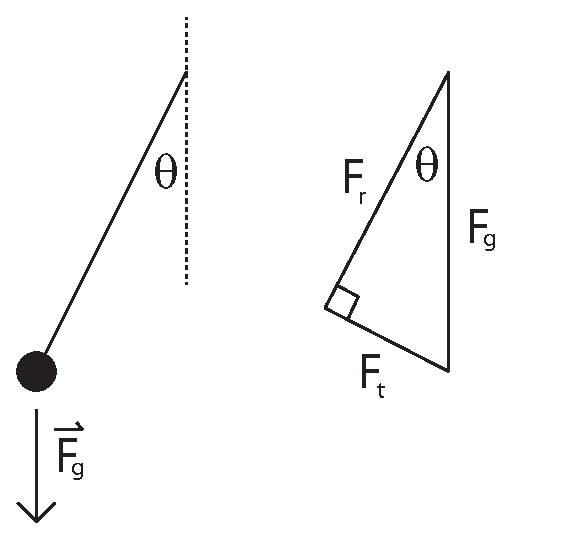
\includegraphics[width=3in]{FOM-pendulum/pendulum1.eps}
\end{center}

\hspace{0.125in}
The only external force acting on our pendulum is gravity, denoted by $\vec{F}_g$, which points downward with magnitude $mg$.  Let us decompose this vector into a sum of two vectors: one that is parallel to the rod, $\vec{F}_r$ ($r$ for `radial'); then the other vector, which we denote by $\vec{F}_t$, must be tangential to the path of the swinging mass.  For a given value of $\theta$, this decomposition is unique.  Trigonometric considerations tell us that 
\[ |\vec{F}_r| = |\vec{F}_g|\cos(\theta) \ \ \ \mbox{and} \ \ \ |\vec{F}_t | = |\vec{F}_g| \sin(\theta)|.\]
The tangential force $\vec{F}_t$ causes an acceleration of the mass along the circular path centered at the pendulum's fixed point.  We know from precalculus that the linear velocity of the mass is equal to the radius of the circle multiplied by the angular velocity, i.e., $L\dot{\theta}$.  Differentiating this expression gives us the acceleration, $L\ddot{\theta}$.  Newton's second law then tells us that the tangential force equal the mass times the acceleration:
\[ mL \ddot{\theta} = -mg\sin(\theta).\]
\end{minipage}
}
\end{center}

\newpage
\begin{center}
\psframebox[style=fombox]{\begin{minipage}{6in}
\hspace{0.125in}
Notice the negative sign on the right side of the equation: it is there because the direction of the acceleration will be opposite the direction of the displacement from $\theta=0$, since gravity will work to bring the mass back toward that position.  Dividing through by $m$ and rearranging terms gives us the differential equation
\[ \ddot{\theta}+\frac{g}{L}\sin(\theta)=0.\]

\hspace{0.125in}
There were three important assumptions made in deriving this model:
\begin{enumerate}
\item the rod remains taught and straight;
\item the pendulum moves in only two dimensions; and
\item the motion is not subject to resistance or friction.
\end{enumerate}
Even with these simplifications, the resulting differential equation is not simple to solve.  It can be analyzed using numerical or Taylor methods.  But in order to obtain analytic solutions, we usually make one more assumption: {\it the angle $\theta$ remains small.}  The point of this assumption is that, when $\theta$ is small, $\sin(\theta)\approx \theta$ (provided $\theta$ is measured in radians) which can be seen by neglecting the non-linear terms in the power series representation of sine: $\sin(\theta) = \sum_{n=0}^\infty \frac{(-1)^n \theta^{(2n+1)}}{(2n+1)!} = \theta - \frac{\theta^3}{3!}+\frac{\theta^5}{5!}- \cdots.$  Replacing $\sin(\theta)$ with $\theta$ gives us the simpler, approximate differential equation:
\[ \ddot{\theta} + \frac{g}{L}\theta=0.\]
This second-order linear differential equation can be solved analytically using the methods we will discuss in Chapter 7.

\end{minipage}
}
\end{center}

